\chapter{Experimental apparatus}
\label{Chap:CMS}
In this chapter, the overview of the Large Hadron Collider (LHC) and the Compact Muon Solenoid (CMS) will be introduced. The object reconstruction will be summarized in the last section, as it is closely related to the detectors. 

\section{Large Hadron Collider}
The LHC is so far the largest particle accelerator that human have ever built, and currently hosted by the Europe Organization of Nuclear Research (CERN). 
It possesses a 26.7~km of ring and is placed more than 100~m deep beneath Geneva and France. Such large circumference makes it able to provide high energy collisions, and enables us to examine the validity of the SM and explore the physics such as the existence of the Higgs boson, supersymmetry particles (SUSY), extra-dimension, or even dark matter (DM). The ring consists of two individual and parallel beam pipes, in which protons (or heavy-ions) circulate in opposite directions. 

The protons are grouped together into 2808 bunches, and each bunch contains $1.15\ten{11}$ protons. The time interval between two bunches is 25\unit{ns}, corresponding to a collision rate of 40\unit{MHz}.
A series of machines then successively accelerate and bring proton beams to higher energy. Each beam is accelerated up to an energy of 6.5\TeV when it finally arrives at the LHC beam line. 
%The history of proton beams in the pre-acceleration stage is briefly described below: 
%\begin{itemize}
%\item Protons are obtained by stripping the electrons off the hydrogen atoms which are taken from the hydrogen contained in a bottle.
%\item Protons are injected to the Linear Accelerator (LINAC2) and accelerated to an energy of 50\MeV. 
%\item The Proton Synchrotron Booster (PSB) accelerates the protons from the LINAC2 to 1.4\GeV. 
%\item The PSB feeds the protons to the Proton Synchrotron (PS), where the protons are accelerated to 25\GeV. 
%\item The energy of the protons is brought up to 450\GeV by the Super Proton Synchrotron (SPS). The protons will then be split into two beams, one in a clockwise and the other in an anticlockwise direction, and transferred to the LHC. 
%\item In the LHC beam line, the beams are both accelerated to 6.5\TeV. 
%\end{itemize}

\begin{figure}[!ht]
  \begin{center}
    \includegraphics[width=0.95\textwidth]{Fig/Cern_Complex}\\
    \caption{The CERN accelerator complex. The protons are accelerated from the LINAC2, PSB, PS, SPS, and finally to LHC~\cite{Mobs:2197559}.}
    \label{fig:cerncomp}
  \end{center}
\end{figure}

Fig.~\ref{fig:cerncomp} shows the whole system of the CERN complex~\cite{Mobs:2197559}. 
%There are four intersections where experiments are located, as shown in four yellow points in Fig.~\ref{fig:cerncomp}. Particle beams are focused by quadrapole magnets to collide here. \textbf{A Toroidal LHC Apparatus (ATLAS)} and \textbf{Compact Muon Solenoid (CMS)} are two general purpose detector aiming at looking for the Higgs boson, searching for any possible signature of new physics, and probing the physics in the \TeV scale. These two experiments are complementary on extending the physical reach and providing the mutual evidence of findings. \textbf{LHC-beauty (LHCb)} is a specialized detector for b-physics (``b'' stands for bottom, or beauty, quarks), for which scientists believe that by measuring the properties of charge-conjugate and parity (CP) in decays of these heavy-flavor particles, it may reveal some useful clues as to the matter-antimatter asymmetry in our universe.  \textbf{A Large Ion Collider Experiment (ALICE)} is dedicated to heavy-ion physics (such as lead-lead collisions, or the xenon-xenon collisions that recently performed). The quark–gluon plasma can be produced in heavy-ion collisions, and its properties are key ingredients to understand the origin of color confinement in quantum chromodynamics (QCD). 

An important quantity in the collider physics is the luminosity $\Lumi$. The instantaneous luminosity is defined as:
\begin{equation}
	\frac{\mathrm d N}{\mathrm d t}=\sigma_{\text{event}}\frac{\mathrm d \Lumi}{\mathrm d t}
\end{equation}
The $\frac{\mathrm d N}{\mathrm d t}$ is the event production rate, and $\sigma_{\text{event}}$ is the interaction cross section.
The integrated luminosity $\Lumi_{\text{Tot}}$ is the integral of the instantaneous luminosity over a period of time and a measure of the amount of data. Fig.~\ref{fig:IntegratedLumi} shows the integrated luminosity that CMS recorded in each data-taking year~\cite{CMSLUMI}. 

\begin{figure}[!ht]
  \begin{center}
    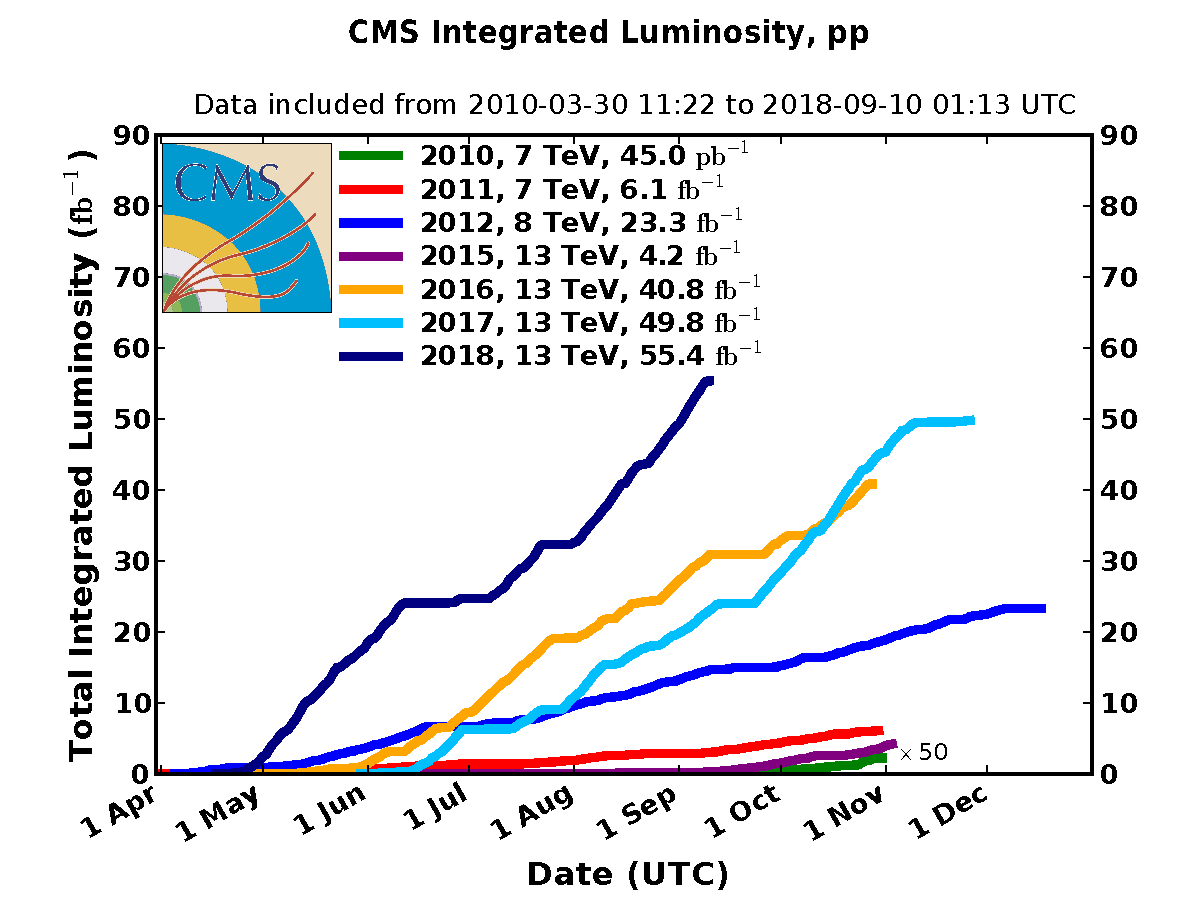
\includegraphics[width=0.95\textwidth]{Fig/int_lumi_cumulative_pp_2}\\
    \caption{Cumulative luminosity versus day delivered to CMS during stable beams for pp collisions at nominal center-of-mass energy. This is shown for data-taking in 2010 (green), 2011 (red), 2012 (blue), 2015 (purple), 2016 (orange), 2017 (light blue), and 2018 (deep blue)~\cite{CMSLUMI}. \label{fig:IntegratedLumi}}
  \end{center}
\end{figure}

\section{Compact Muon Solenoid}
Compact Muon Solenoid is one of the general purpose detectors located at the LHC ring. 
%A detailed description of the CMS detector, together with a definition of the coordinate system used and the relevant kinematic variables, can be found in~\cite{CMS-Jinst}.
The central feature of the CMS apparatus is a superconducting solenoid of 13\unit{m} in length and 6\unit{m} in internal diameter, providing an axial magnetic field of 3.8\unit{T}. Within the solenoid volume are a silicon pixel and strip tracker, a lead tungstate crystal electromagnetic calorimeter (ECAL), and a brass and scintillator hadron calorimeter (HCAL), each composed of a barrel and two endcap sections. Forward calorimeters extend the pseudorapidity ($\eta$) coverage provided by the barrel and endcap detectors. Muons are detected in gas-ionization chambers embedded in the steel flux-return yoke outside the solenoid. 

The adopted coordinate system, as shown in Fig.~\ref{fig:cmscoordinate}, has the origin at the nominal collision point inside CMS detector, where the y-axis pointing vertically upward, the x-axis pointing radially inward toward the center of the LHC, and the z-axis pointing along the beam direction. The azimuthal angle $\phi$ is measured from the x-axis in the x-y plane, while the polar angle $\theta$ is measured from the z-axis. 
Rapidity, $\mathit{Y}$, is defined as $\mathit{Y}\equiv\frac{1}{2}\ln\big(\frac{E+p_{z}c}{E-p_{z}c}\big)$, where $E$ is the energy of the particle and $p_{z}$ is the momentum in the z direction.
This Lorentz invariant quantity indicates the angle between the x-y plane and the direction of the measured particle.
For the highly relativistic particles, the other quantity called pseudorapidity, defined as $\eta = -\ln \tan(\theta /2)$, is used, where $\theta$ is the angle between the particle trajectory and the z-axis (beam pipe).

\begin{figure}[!ht]
  \begin{center}
    \includegraphics[width=1.0\textwidth]{Fig/cms_coordinate}\\
    \caption{The adopted coordinate system in CMS. \label{fig:cmscoordinate}}
  \end{center}
\end{figure}

The momentum and energy transverse to the beam direction, denoted by $\pt$ and $\et$ , respectively, are computed from the x and y components.

\begin{figure}[!ht]
  \begin{center}
    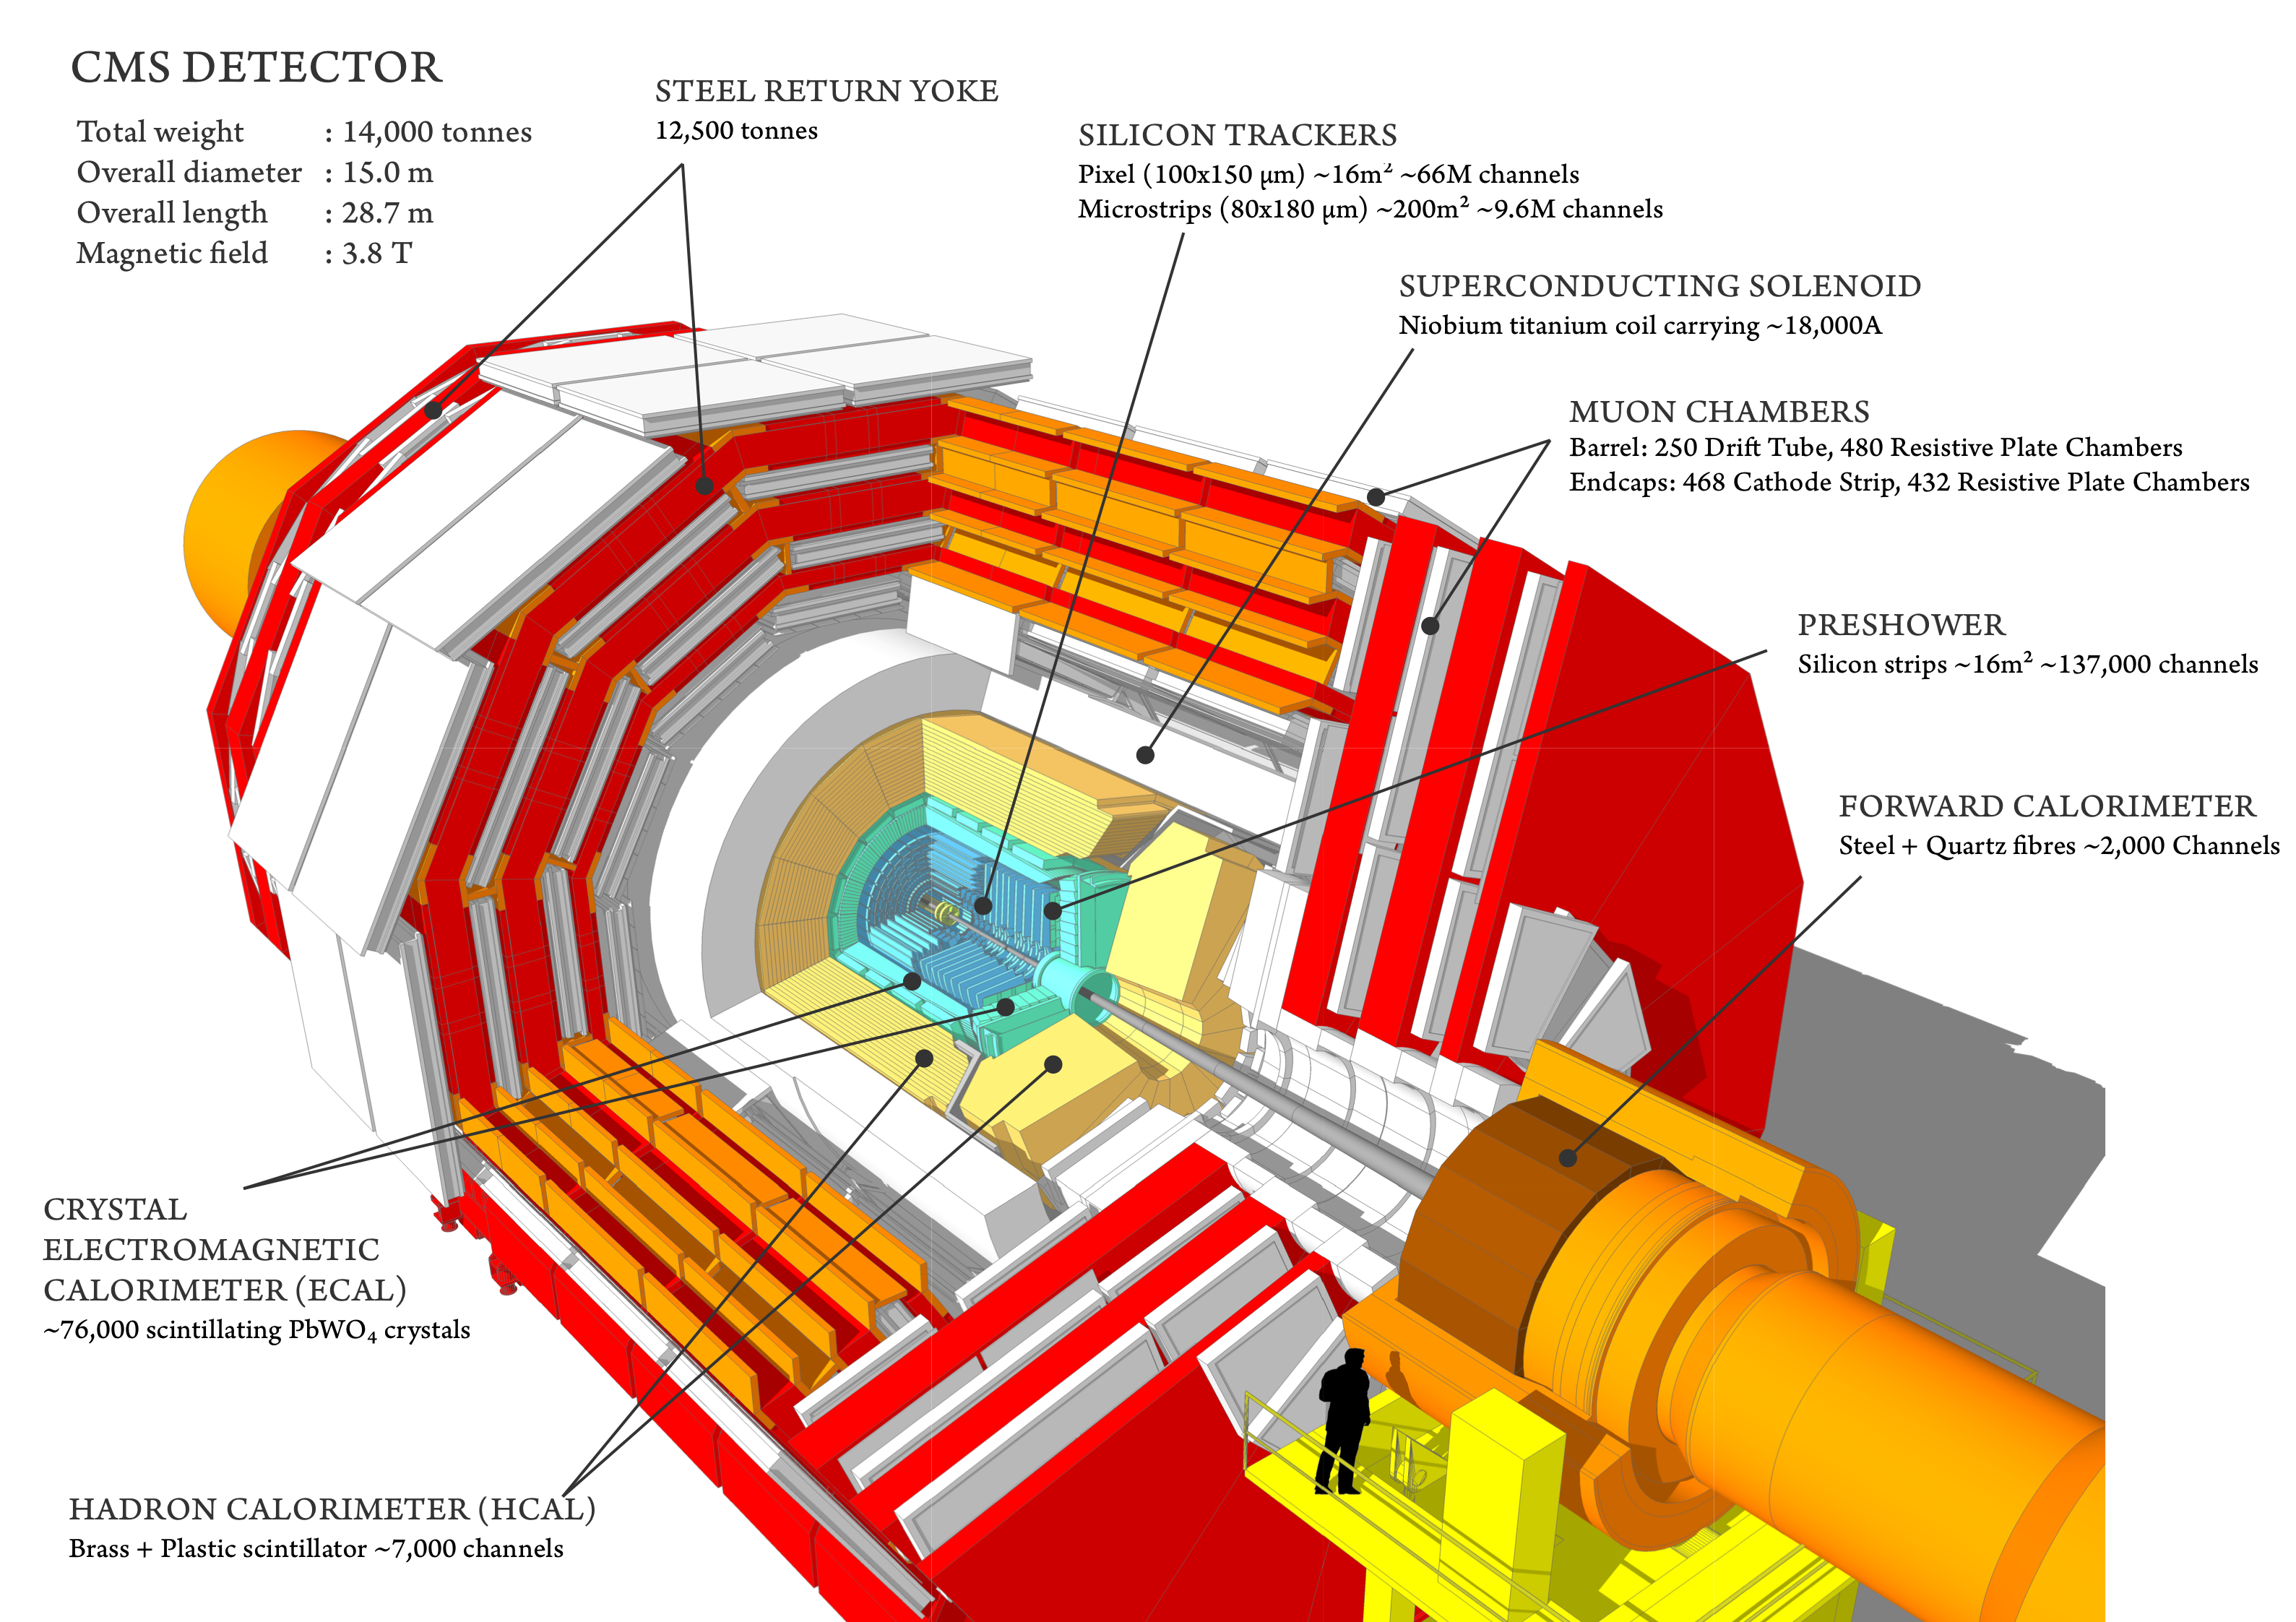
\includegraphics[width=0.85\textwidth]{Fig/cms_120918_03}\\
    \caption{A cutaway view of the CMS detector~\cite{Sakuma:1626816}. \label{fig:CMSdetector}}
  \end{center}
\end{figure}
Fig.~\ref{fig:CMSdetector} shows a global view of the CMS detector~\cite{Sakuma:1626816}. Brief description of each sub-detector is summarized as follows.

\subsection*{Superconduction magnet}
The superconducting solenoid magnet, formed by a cylindrical coil of superconducting fibers, was originally designed to provide a magnetic field of 4 Tesla (T), while in the actual operation it produces a 3.8\unit{T} of field. Such large bending power enables us to measure the momentum of high energy charged particles precisely. 
The magnetic field is confined to the volume of the detector. This is done by the steel yoke, consisting of five layers for barrel part and three layers for each endcap. 
\subsection*{Silicon tracker}
The CMS tracker is composed of two systems: a pixel detector (for a total of 1440 silicon pixel modules) with three barrel layers, and a silicon strip tracker (for a total of 15148 silicon strip modules) with ten barrel detection layers, four layers of tracker inner barrel (TIB) and six layers of tracker outer barrel (TOB), extending outwards. 
Each system is completed by endcaps, which consist of two disks in the pixel detector, three tracker inner disks (TID) and nine disks of tracker endcaps (TEC) in the strip tracker on each side of the barrel. The acceptance of the whole tracker system extends up to a $|\eta|<2.5$. 
Fig.~\ref{fig:TrkerLayout} shows the schematic view of the silicon tracker in the r-z plane. The upper plot is the cross section through the tracker, and the lower one is one quarter of the tracker, where the paths of the laser rays (R), the alignment tubes (A) and the beam splitters (B) of the laser alignment system are illustrated.

For non-isolated particles with transverse momentum, $\pt$, between 1 and 10GeV and $|\eta|<1.4$, the track resolutions are typically 1.5\% in $\pt$ and 25–90 (45–150) $\mu$m in the transverse (longitudinal) impact parameter~\cite{TRK-11-001}.

\begin{figure}[!ht]
  \begin{center}
  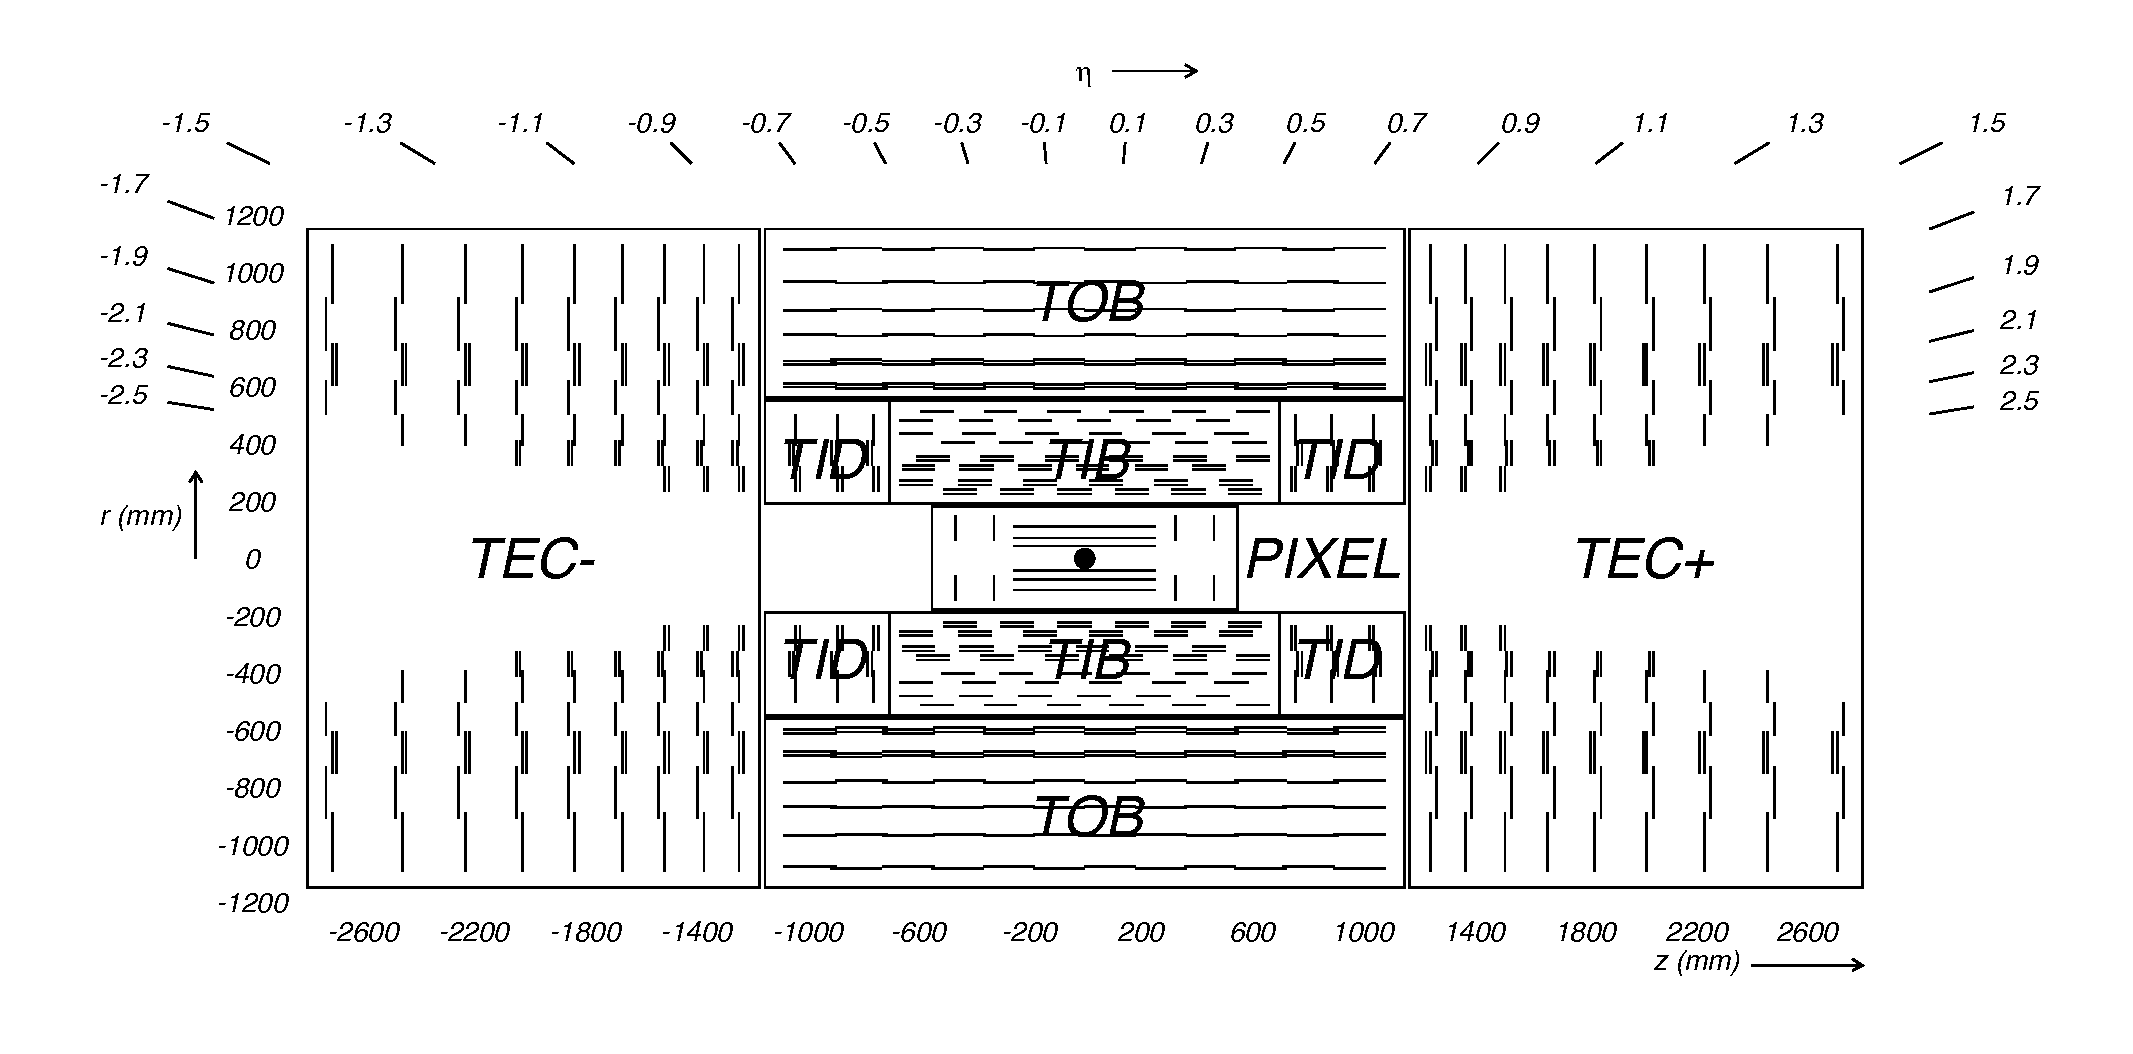
\includegraphics[width=0.7\textwidth]{Fig/CMS_Detector/TrakerLayout}\\
    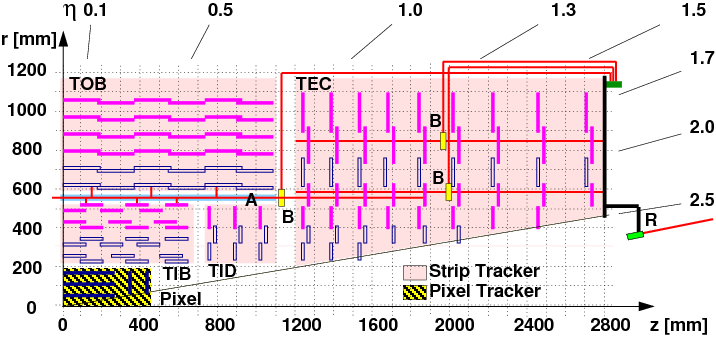
\includegraphics[width=0.6\textwidth]{Fig/CMS_Detector/figs_TrackerLayoutWithLAS}\\
    \caption{Schematic view of one quarter of the silicon tracker in the r-z plane~\cite{Chatrchyan:2008aa}.\label{fig:TrkerLayout}}
  \end{center}
\end{figure}

\subsection*{Electromagnetic calorimeter}
The electromagnetic calorimeter (ECAL) is a homogeneous calorimeter made of 61200 lead tungstate ($\text{PbWO}_{4}$) crystals in the barrel part ($0<|\eta|<1.48$) and 7324 crystals in each of endcaps ($1.48<|\eta|<3.0$). 
The high density ($8.28\unit{g}/\unit{cm}^{3}$) and short radiation length $\text{X}_{0}$\footnotemark ($0.89\unit{cm}$) of the crystal result in a compact calorimeter with fast response, fine granularity, and strong resistance to the radiation. A sampling calorimeter, preshower detector (ES), is placed in front of the endcap crystals and covers the range of $1.65<|\eta|<2.6$.  It consists of two planes of silicon sensors interleaved with a total of 3$\text{X}_{0}$ of lead.
The main task of this detector is to help on distinguishing between single high-energy photons and the close pairs of low-energy photons, usually from the decay of neutral pion. The ES also improves the ability of identifying electrons against minimum ionizing particles and the position determination of electrons and photons . Fig.~\ref{fig:EcalLayout} shows layout of the CMS ECAL.
\footnotetext{One radiation length of a given material is defined as the distance after which the electron loose $1/\mathrm{e}$ of its original energy.}
\begin{figure}[!ht]
  \begin{center}
 	%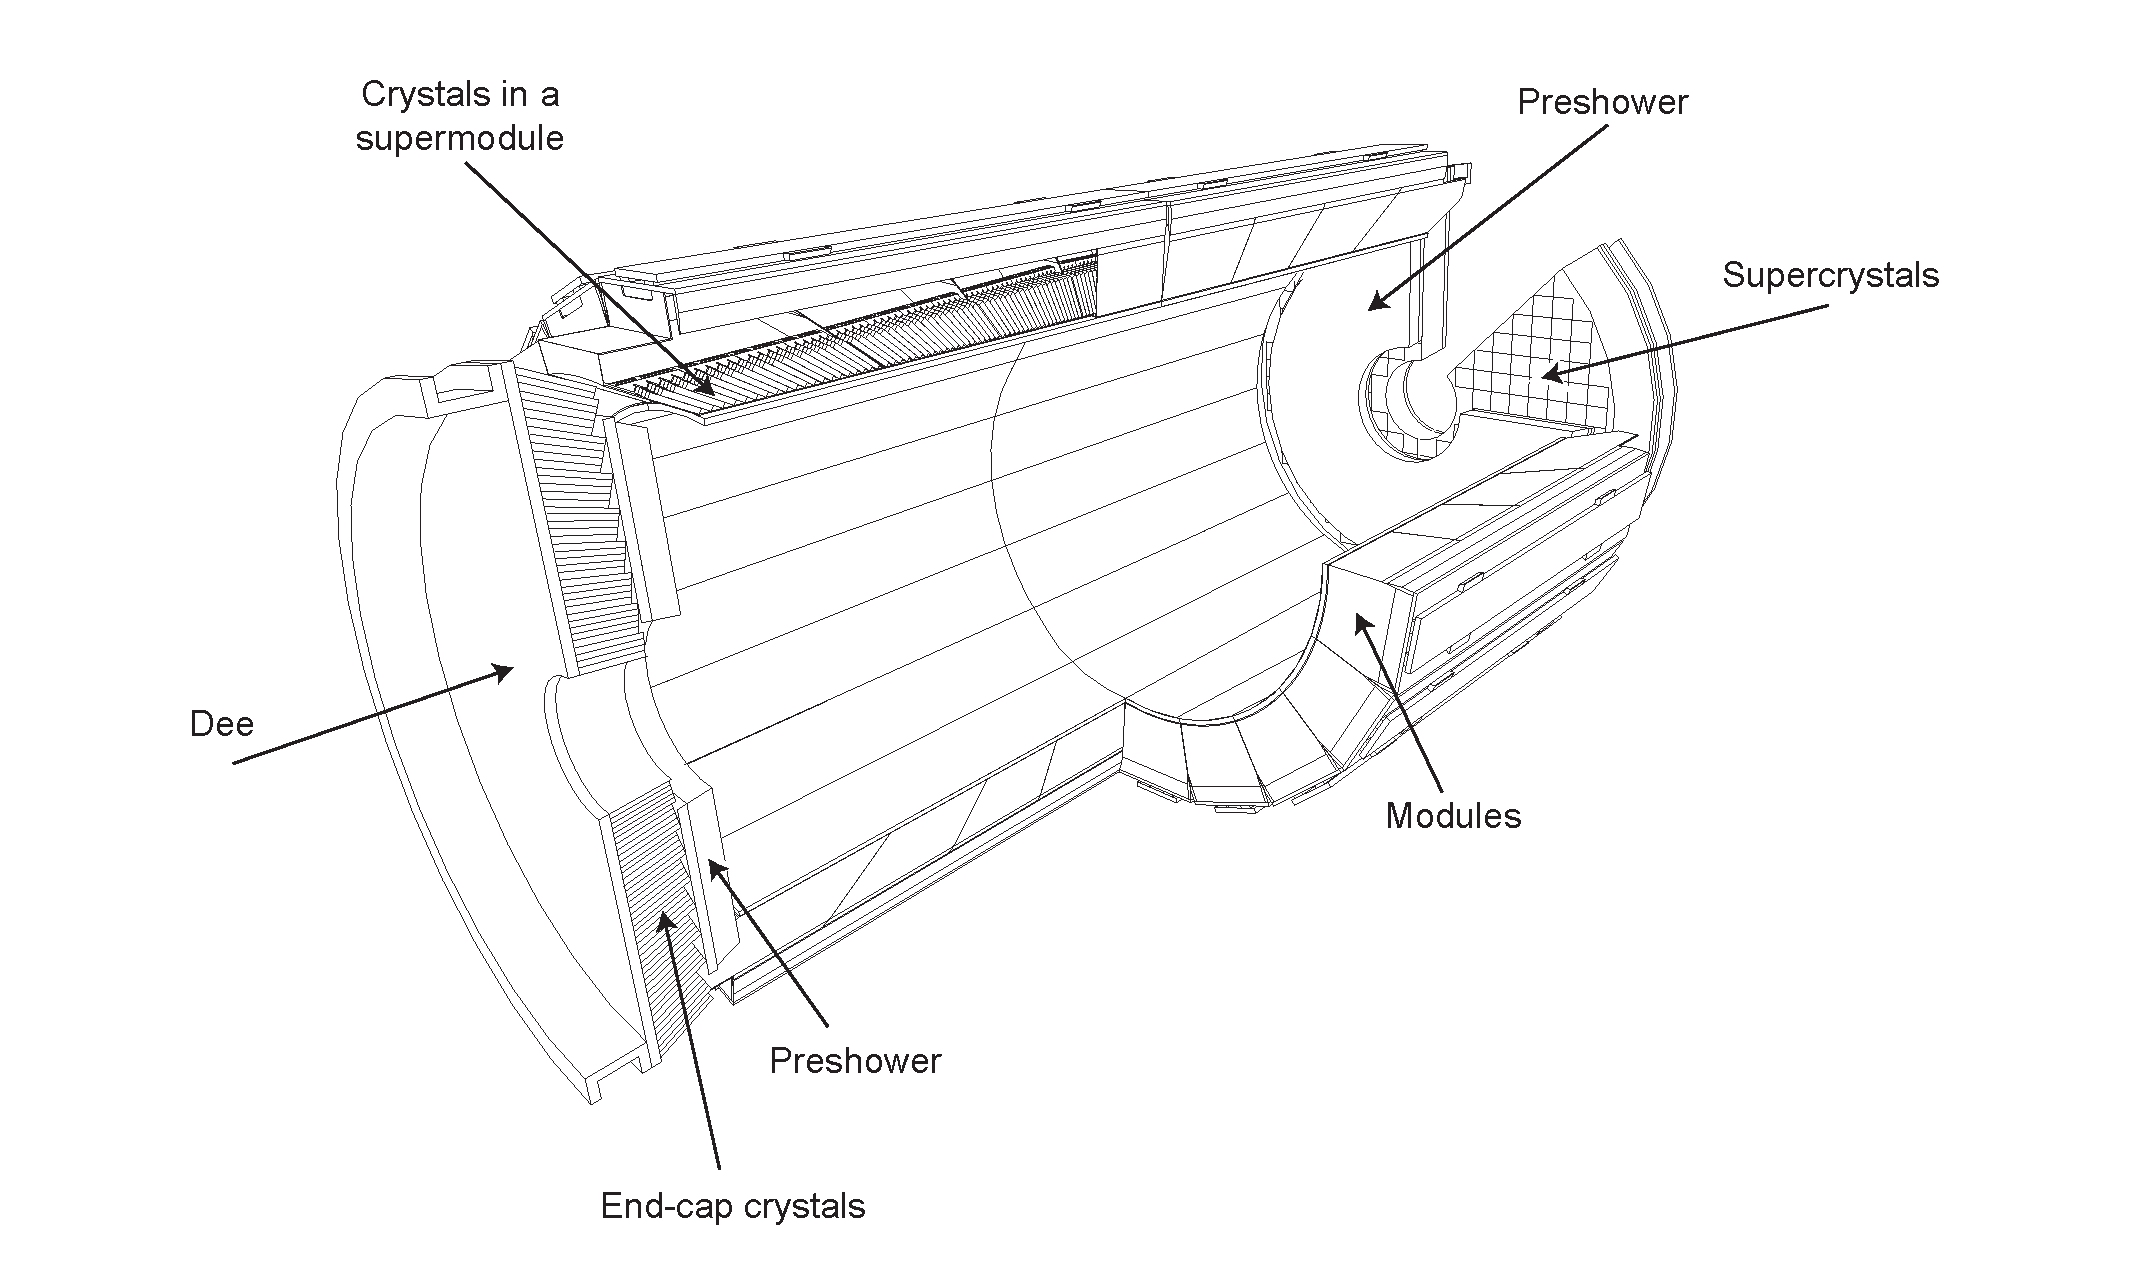
\includegraphics[width=0.75\textwidth]{Fig/CMS_Detector/ECAL_layout}\\
  	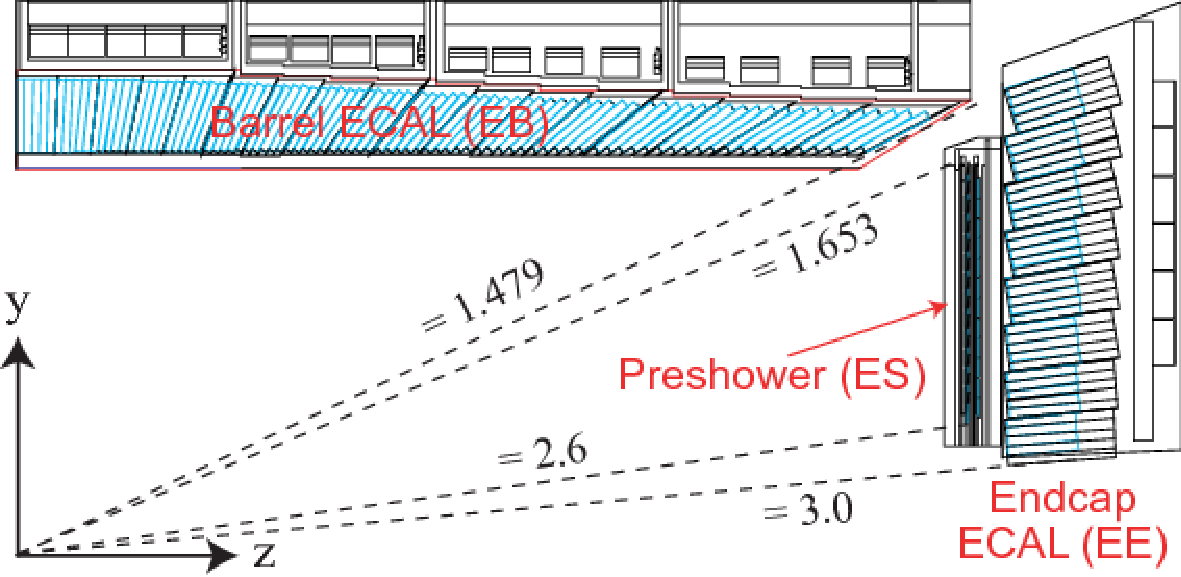
\includegraphics[width=0.7\textwidth]{Fig/CMS_Detector/Figure_004-001}\\
    \caption{Layout of the ECAL~\cite{Benaglia:2014aqa}.}
    \label{fig:EcalLayout}
  \end{center}
\end{figure}

\subsection*{Hadron calorimeter}
The hadron calorimeters (HCAL), a sampling calorimeter, measures the energy of hadron jets and provides indirect measurement of missing transverse energy, which can be neutrinos or exotic particles that do not interact with matters.  
Fig.~\ref{fig:HCalLayout} shows the longitudinal view of the CMS detector with the dashed lines representing fixed $\eta$ values. 
The HCAL consists four parts: the HCAL barrel (HB), the HCAL endcap (HE), the HCAL outer (HO), and the HCAL forward (HF). 
The HB, covering the range of $|\eta|<1.3$, is placed radially between the outer extent of the ECAL and the inner extent of the magnet coil. The HO sits outside the solenoid complementing the barrel part, and ensure the leakage of the energy not detected by HB to be minimal.
The HE covers the range of $1.3<|\eta|<3.0$, a region containing about 34\% of the particles produced in the final state.
The HF is place at the range of $|\eta|>3.0$, where much higher energy will be deposited compared to other sub-detectors.  
\begin{figure}[!ht]
  \begin{center}
  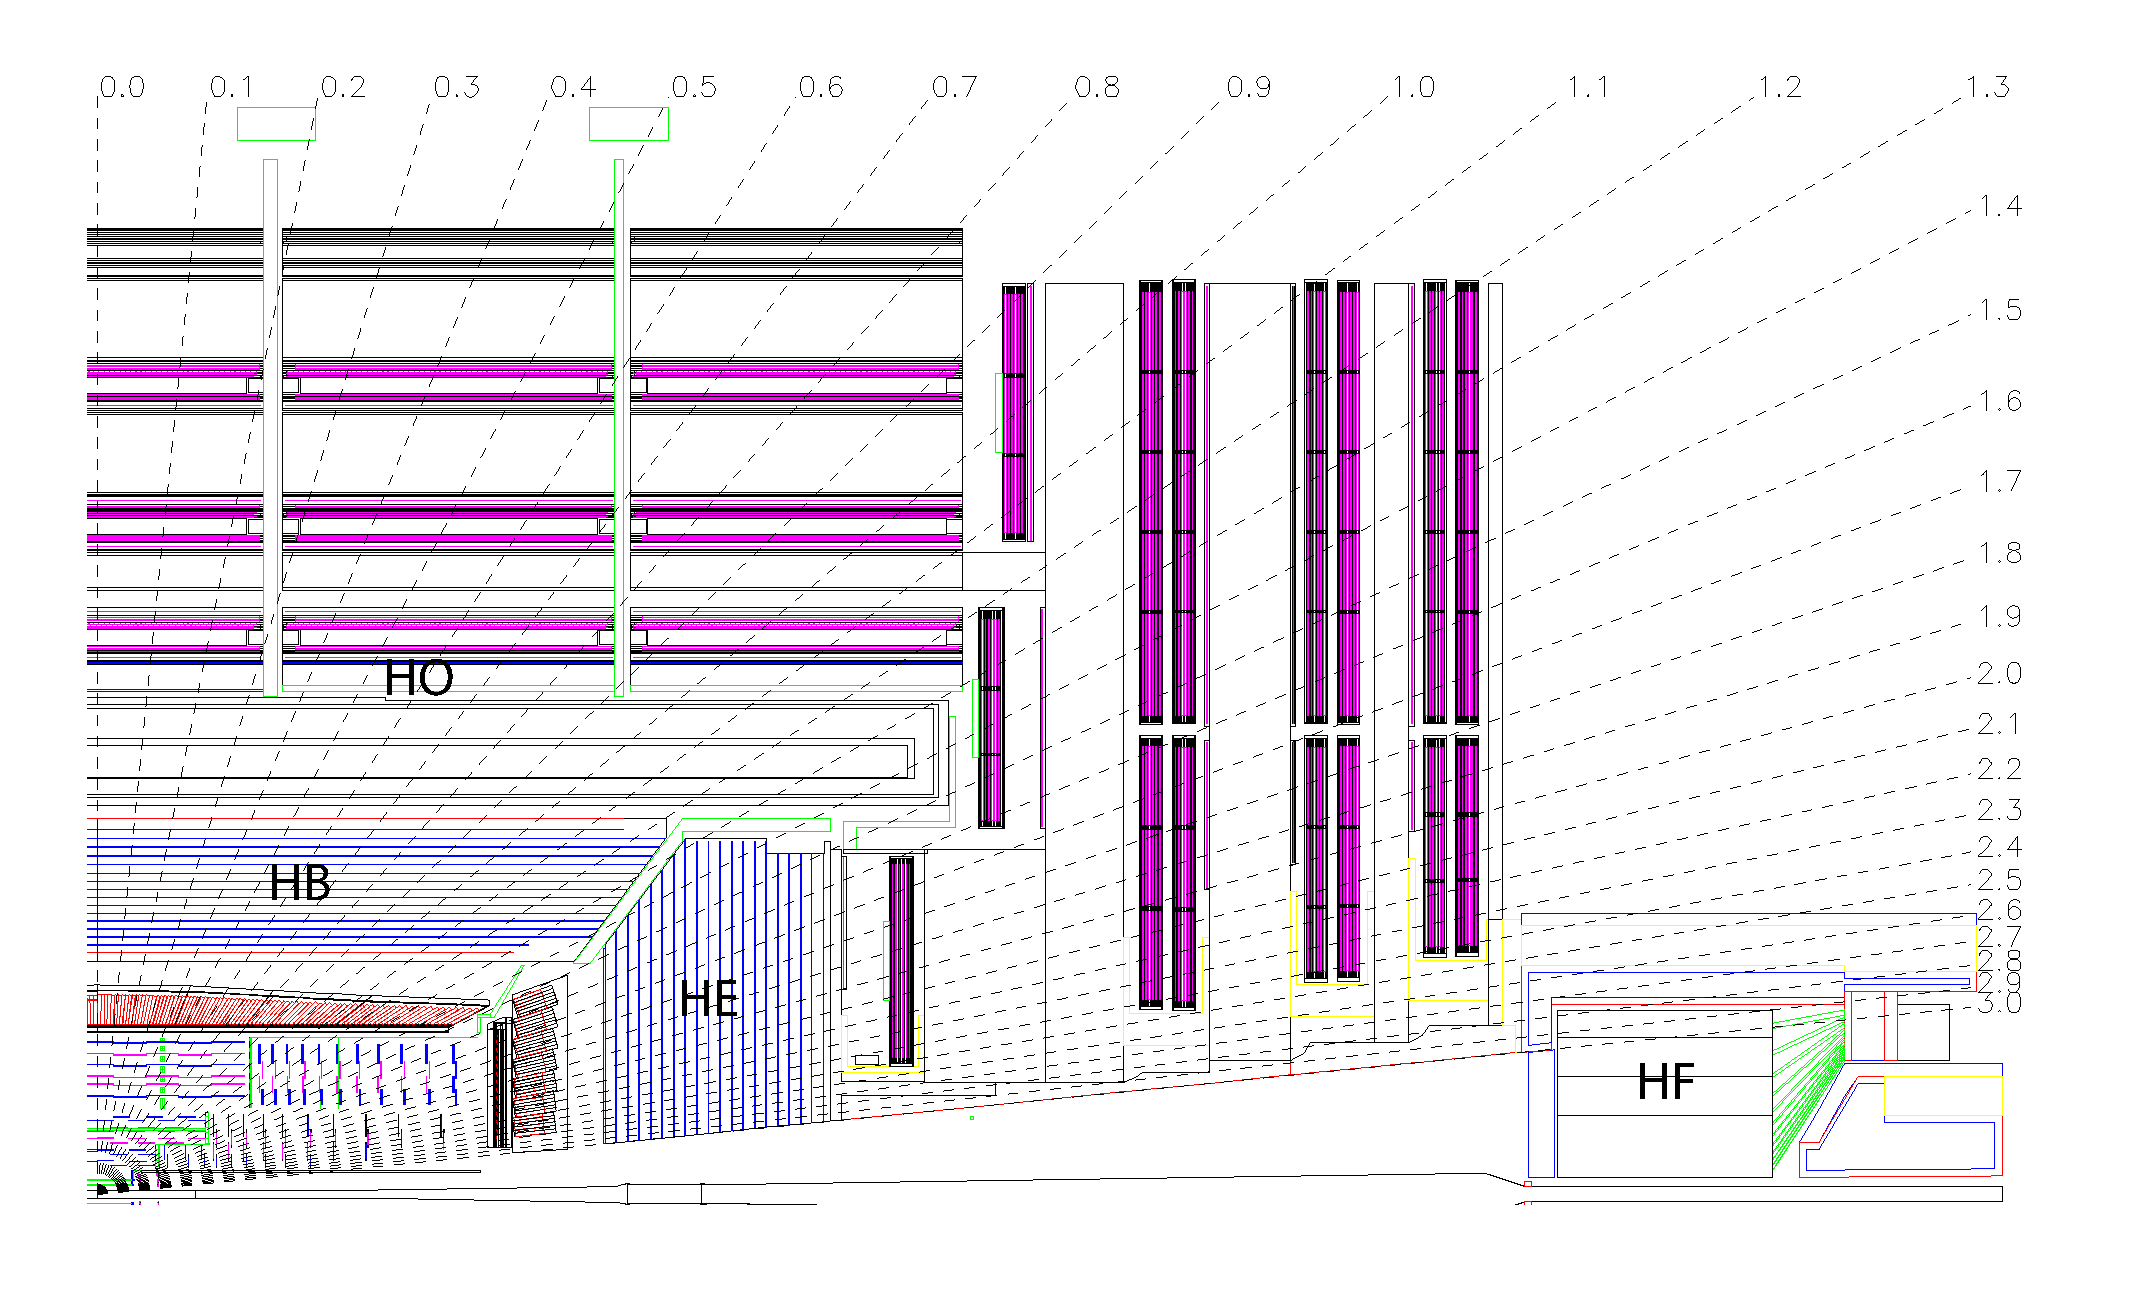
\includegraphics[width=0.7\textwidth]{Fig/CMS_Detector/HCAL_layout}\\
    \caption{Longitudinal view of the CMS detector showing the locations of the hadron barrel (HB), endcap (HE), outer (HO) and forward (HF) calorimeters~\cite{Chatrchyan:2008aa}. \label{fig:HCalLayout}}
  \end{center}
\end{figure}

\subsection*{Muon system}
The muon system is located outside the solenoid and covers the range $|\eta|<2.4$. It is composed of three types of gaseous detectors, drift tubes (DTs), cathode strip chambers (CSCs), and resistive plate chambers (RPCs), sandwiched among the layers of the steel yoke. 
The DTs are segmented into drift cells; the position of the muon is determined by measuring the drift time to an anode wire of a cell with a shaped electric field. 
The CSCs operate as standard multi-wire proportional counters but with a finely segmented cathode strip readout, which yields an accurate measurement of the position of the bending plane $(\text{R}-\phi)$ coordinate at which the muon crosses the gas volume. 
The DT and CSC chambers are located in the regions $|\eta| < 1.2$ and $0.9 < |\eta| < 2.4$, respectively, and are complemented by RPCs in the range $|\eta| < 1.9$. Three regions are defined and referred to as the barrel ($|\eta| < 0.9$), overlap ($0.9 < |\eta| < 1.2$), and endcap ($1.2 < |\eta| < 2.4$) regions~\cite{Sirunyan:2018fpa}. 
Fig.~\ref{fig:MuonSystLayout} shows the arrangement of the muon system. 
\begin{figure}[!ht]
  \begin{center}
  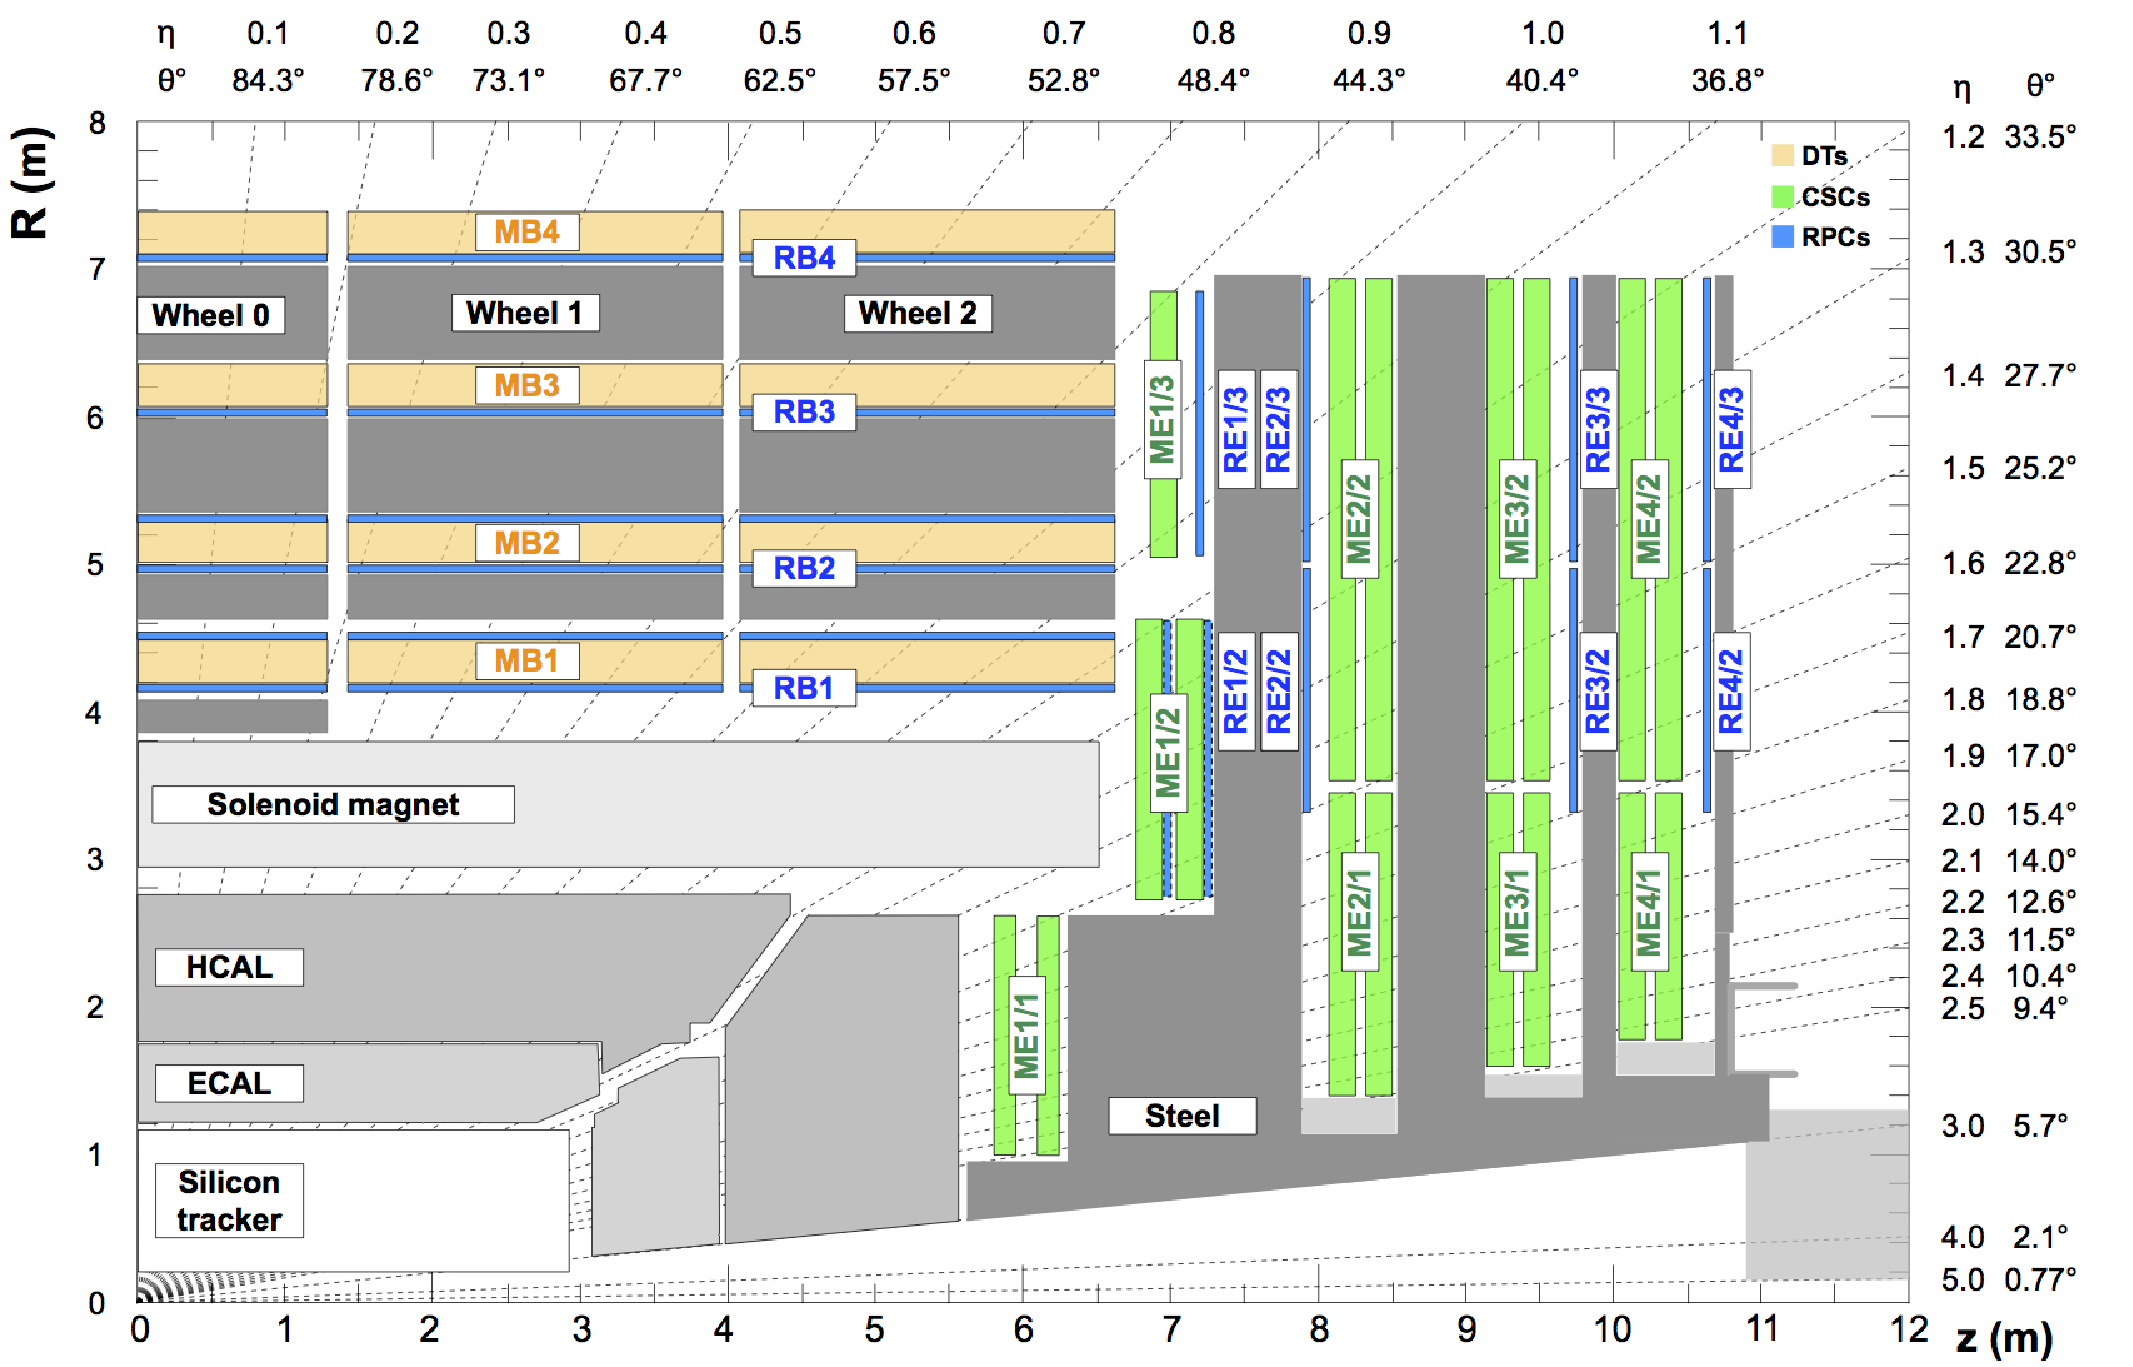
\includegraphics[width=0.7\textwidth]{Fig/CMS_Detector/MuonSystem_layout}
    \caption{An R-z cross section of the muon station. The drift tube stations (DTs) are labeled MB ("Muon Barrel'') and the cathode strip chambers (CSCs) are labeled ME ("Muon Endcap''). Resistive plate chambers (RPCs) are mounted in both the barrel and endcaps of CMS, where they are labeled RB and RE, respectively~\cite{Sirunyan:2018fpa}. \label{fig:MuonSystLayout}}
  \end{center}
\end{figure}

\subsection*{Trigger and data acquisition system}
The LHC provides $\Pp\Pp$ and heavy-ion collisions at high interaction rate. This corresponds to an enormous amount of data that are currently not able to be completely stored. Furthermore, most of these interactions would be low-energy glancing collisions, rather than energetic and head-on interactions where processes of interested may occur. The trigger system is designed to reduce the rate and to start the physics event selection process. Fig.~\ref{fig:TrigSyst} shows the schematic diagram of the trigger architecture and data acquisition system. The level-1 trigger (L1) consists of custom-designed and programmable electronics. Information from muon system (including DTs, CSCs, and RPCs), ECAL, HCAL, and HF is used to reconstruct candidate trigger objects, and these quantities are combined and forwarded to the Global Trigger (GT), which calculates the trigger decision and sends out the signal if it is ''L1 Accept (L1S)``. This step reduces the data rate from the 40 \unit{MHz} of the LHC bunch crossing rate down to a maximum of 100 \unit{kHz}. 
In case of a positive L1 decision all data for the corresponding bunch crossing time is read out from the CMS detector and transferred to the HLT, which consists of a software system implemented in a filter farm. The high level trigger algorithm (HLT) performs a full reconstruction of events using a faster version of offline software and writes data out to permanent storage at a typical rate of several hundred \unit{Hz}.
\begin{figure}[!ht]
  \begin{center}
  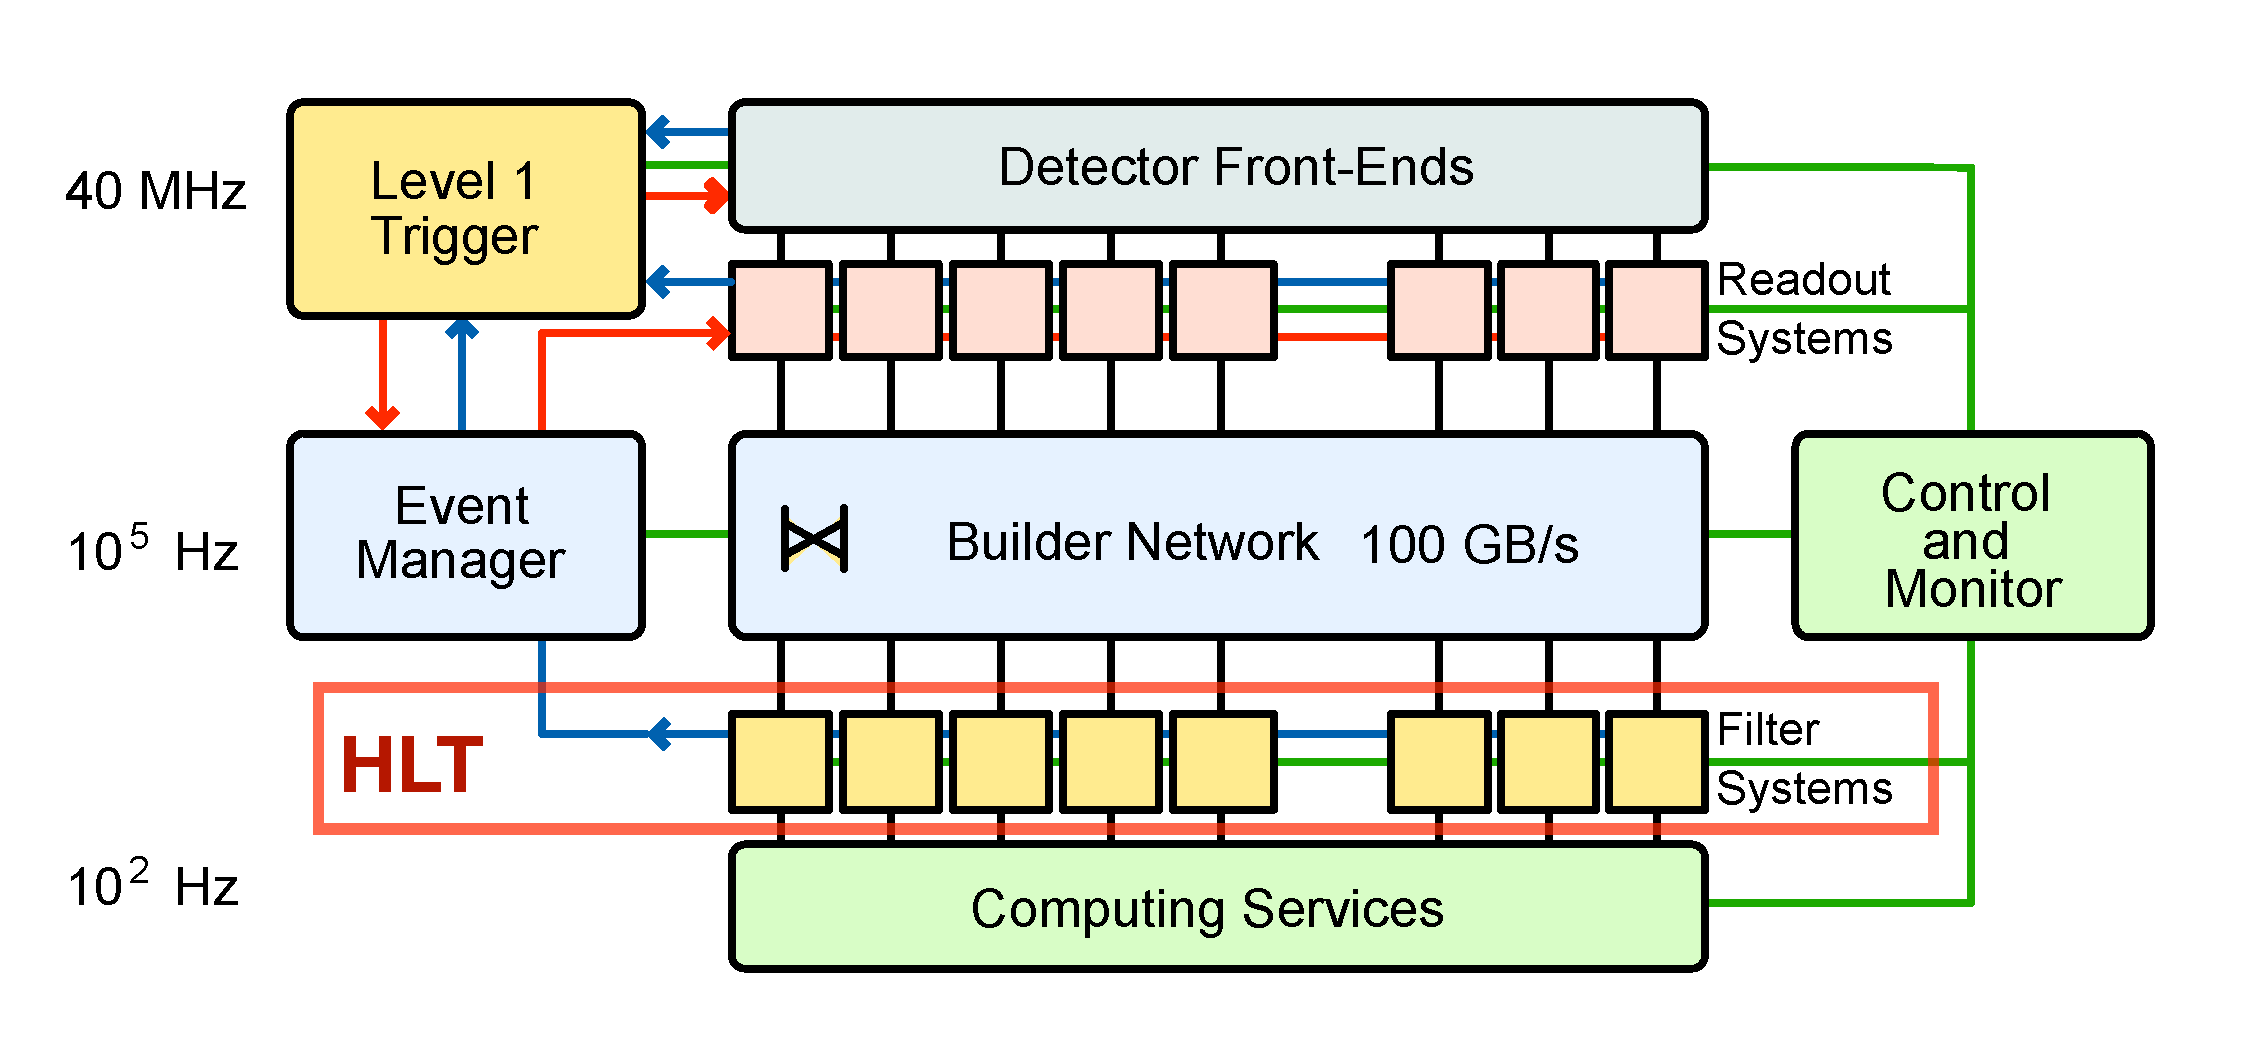
\includegraphics[width=0.8\textwidth]{Fig/CMS_Detector/Trigger_architexture}
    \caption{A schematic diagram of the trigger system~\cite{Chatrchyan:2008aa}. \label{fig:TrigSyst}}
  \end{center}
\end{figure}

\section{Object reconstruction}
	\subsection{Particle-Flow algorithm}
%		The PF algorithm event reconstruction was originally developed and used in the ALEPH (Apparatus for LEP PHysics) experiment at LEP, which collided electron and positron beams. 
		The core concept of this algorithm is to optimally correlate tracks or clusters from all sub-detectors and combines the information to reconstruct final state particles. In order to have PF algorithm as efficient as possible, the magnetic field should be strong enough to maximize the separation between charged and neutral particles, and the detector should have fine spatial granularity layers that can distinguish merged particles, especially those in jets. The CMS meets all of these advantages to use PF reconstruction as a global event description. 
%		However, the remnant of the collisions, additional pile-up interactions, the proximity of particles inside an energetic jet, and the interactions in the detector materials dramatically increase the multiplicity and complexity of the final state particles in $\Pp\Pp$ or heavy-ion collisions, and may spoil the quality of the PF reconstruction. Dedicated simulation and commissioning of the data collected during the first few weeks of $\sqrt{s}=7\TeV$ collisions were done, and showed that the performance was not severely degraded. The robustness of the PF algorithm was then widely demonstrated and validated, the usage was therefore confirmed. 

		The ECAL energy clusters without being associated to extrapolated tracks from tracker are reconstructed as photons. Electrons are reconstructed by tracks in the tracker system with associated energy deposits in the ECAL. The bremsstrahlung emission and energy losses when traveling through tracker materials are properly accounted for. Muons tracks can be reconstructed in tracker, in muon system, or the combination of the two. Charged hadrons are reconstructed by the tracks not identified as electrons or muons with energy cluster in HCAL. The energy clusters that correspond to excesses of energy with respect to charged hadrons and not linked to charged particle trajectories are reconstructed as neutral hadrons. 

		In this analysis, photon and muons are selected as final states particles. Hence, their reconstructions are described in detail in the following paragraphs.

\subsection*{Photon reconstruction}
		Photons are reconstructed from energy deposits in the ECAL. The algorithms, without any hypothesis as to whether the particle from the interaction point is a photon or an electron, identify the energy clusters and constrains them to the expected sizes and shapes, based on the study of simulation. The measurements of photon trigger, reconstruction, and identification efficiencies and energy scale and resolution can therefore utilize the electrons from $\cPZ\to e^{+}e^{-}$ events with a well defined invariant mass. 
		
		The clustering algorithms are used to sum over all energy deposits in crystals in the same electromagnetic shower. A basic cluster (BC) is chosen to be the local maximum among the energy deposits. Several BCs are combined to construct a supercluster (SC). The radiated energies, such as the conversions of photons or bremsstrahlung from electrons, are corrected and recovered for their corresponding SC.
		The energy of the photon is determined by summing the amplitude in channels $\mathit{A_{i}}$ over the crystals $i$ in the supercluster where the photon leaves energy, corrected by the intercalibration $\mathit{c_{i}}$ and light monitoring $\mathit{S_{i}(t)}$ constants. The procedure can be summarized in a formula,
		\begin{equation}
		\mathit{E_{\gamma}} = \bigg[ \sum_{i} \bigg(\mathit{S_{i}(t)} \times \mathit{c_{i}} \times \mathit{A_{i}}\bigg) \times \mathit{G}(\eta) + \mathit{E_{ES}} \bigg] \times \mathit{F_{\gamma}}
		\end{equation}
	where $\mathit{G}(\eta)$ is the ADC to \GeV factor. 
		
		Independent methods are used to calculate the intercalibration constants (ICs), and the combined factor is obtained from the mean of the individual IC at a fixed value of $\eta$, weighted by their respective precisions. A light monitoring system, consisting of a system of lasers that inject light to crystals, is used to monitor the time dependence of response in the ECAL resulting from the decreases in crystal transparency in radiation exposure. The difference between input and read laser amplitudes are then used to calculate correction factors $\mathit{S_{i}(t)}$.
		For photon in the region $1.65<|\eta|< 2.6$ the energy deposits in the preshower $\mathit{E_{ES}}$ are also accounted for. 
		The cluster corrections $\mathit{F_{\gamma}}$ is applied to take the variation of shower containment in the clustered crystals and the shower losses of photons that convert before reaching the calorimeter into account. The correction factors are computed with a multivariate regression technique that estimates the energy of the photon and its uncertainty simultaneously. The resolution of photon energy is optimized after applying the factors.
		
		The ECAL energy resolution was measured in beam tests, and found to be:
		\begin{equation}
		\frac{\sigma_{E}}{E}=\frac{2.8\%}{\sqrt{E\ (GeV)}} \oplus \frac{12\%}{E\ (GeV)} \oplus 0.3\%.
		\end{equation}
		The first contribution is the stochastic term, which represents the event to event fluctuations in the lateral shower containment.
		The second term comes from the electronic noise. The last one is the constant term, characterizing the resolution at high energy region. 

	 		The energy scale and resolution is further measured and calibrated using a high purity $\cPZ\to\EE$ samples with 2\% of background contamination, estimated from simulation. An unbinned maximum likelihood fit to the invariant mass distribution is performed. A Breit-Wigner distribution convolved with a Crystal Ball (CB) function~\cite{CBall} is used.
	 	\begin{equation}
			\label{eq:bwcb}
			CB(m-\Delta m)=
				\begin{cases}
				e^{-\frac{1}{2}(\frac{m-\Delta m}{\sigma_{CB}})^2 },& \frac{m-\Delta m}{\sigma_{CB}}>\alpha\\
				\bigl(\frac{\gamma}{\alpha}\bigr)^\gamma\cdot e^{-\frac{\alpha^2}{2}}
				\cdot\biggl(\frac{\gamma}{\alpha}-\alpha-
				\frac{m-\Delta m}{\sigma_{CB}}\biggr)^{-\gamma}, & \frac{m-\Delta m}{\sigma_{CB}}<\alpha  \\
				\end{cases}
	\end{equation}
	where the parameter $\Delta m$ quantifies the displacement of the peak with respect to the nominal $\cPZ$ boson mass; $\sigma_{CB}$ is the the width of the Gaussian component of the CB function and serves as a measure of the energy resolution; the parameters $\alpha$ and $\gamma$ describe the tail part of CB, accounting for electrons of which energy is not fully retained after the clustering algorithms. In this step, the ADC to \GeV factor $\mathit{G}(\eta)$ is also adjusted and determined such that the peak value from the fit to $\cPZ\to \EE$ distribution agrees with that of the simulation, independently for the barrel and endcap. There are still unknown effects that make the resolution of $\cPZ\to\EE$ distribution in data worse than that in simulation. These residual discrepancies are corrected by adding a Gaussian smearing, where the parameters of smearing function are determined by a comparison between the lineshapes of $\cPZ\to\EE$ in data and simulation.  
	As a result, the corrections to the energy scale vary in time, $|\eta|$ and $\RNINE$ variable, which is defined as the energy sum of the $3\times3$ crystals centered on the most energetic crystal in the candidate electromagnetic cluster divided by the energy of the candidate. The amount of smearing required changes from about 0.1\% to about 2.7\%, depending on the same categories as the energy scale corrections.
	The comparison of the dielectron invariant mass distributions in data and simulation after energy smearing are shown in Fig.~\ref{fig:ZeeComp}. 
		\begin{figure}[!ht]
		  \centering
		  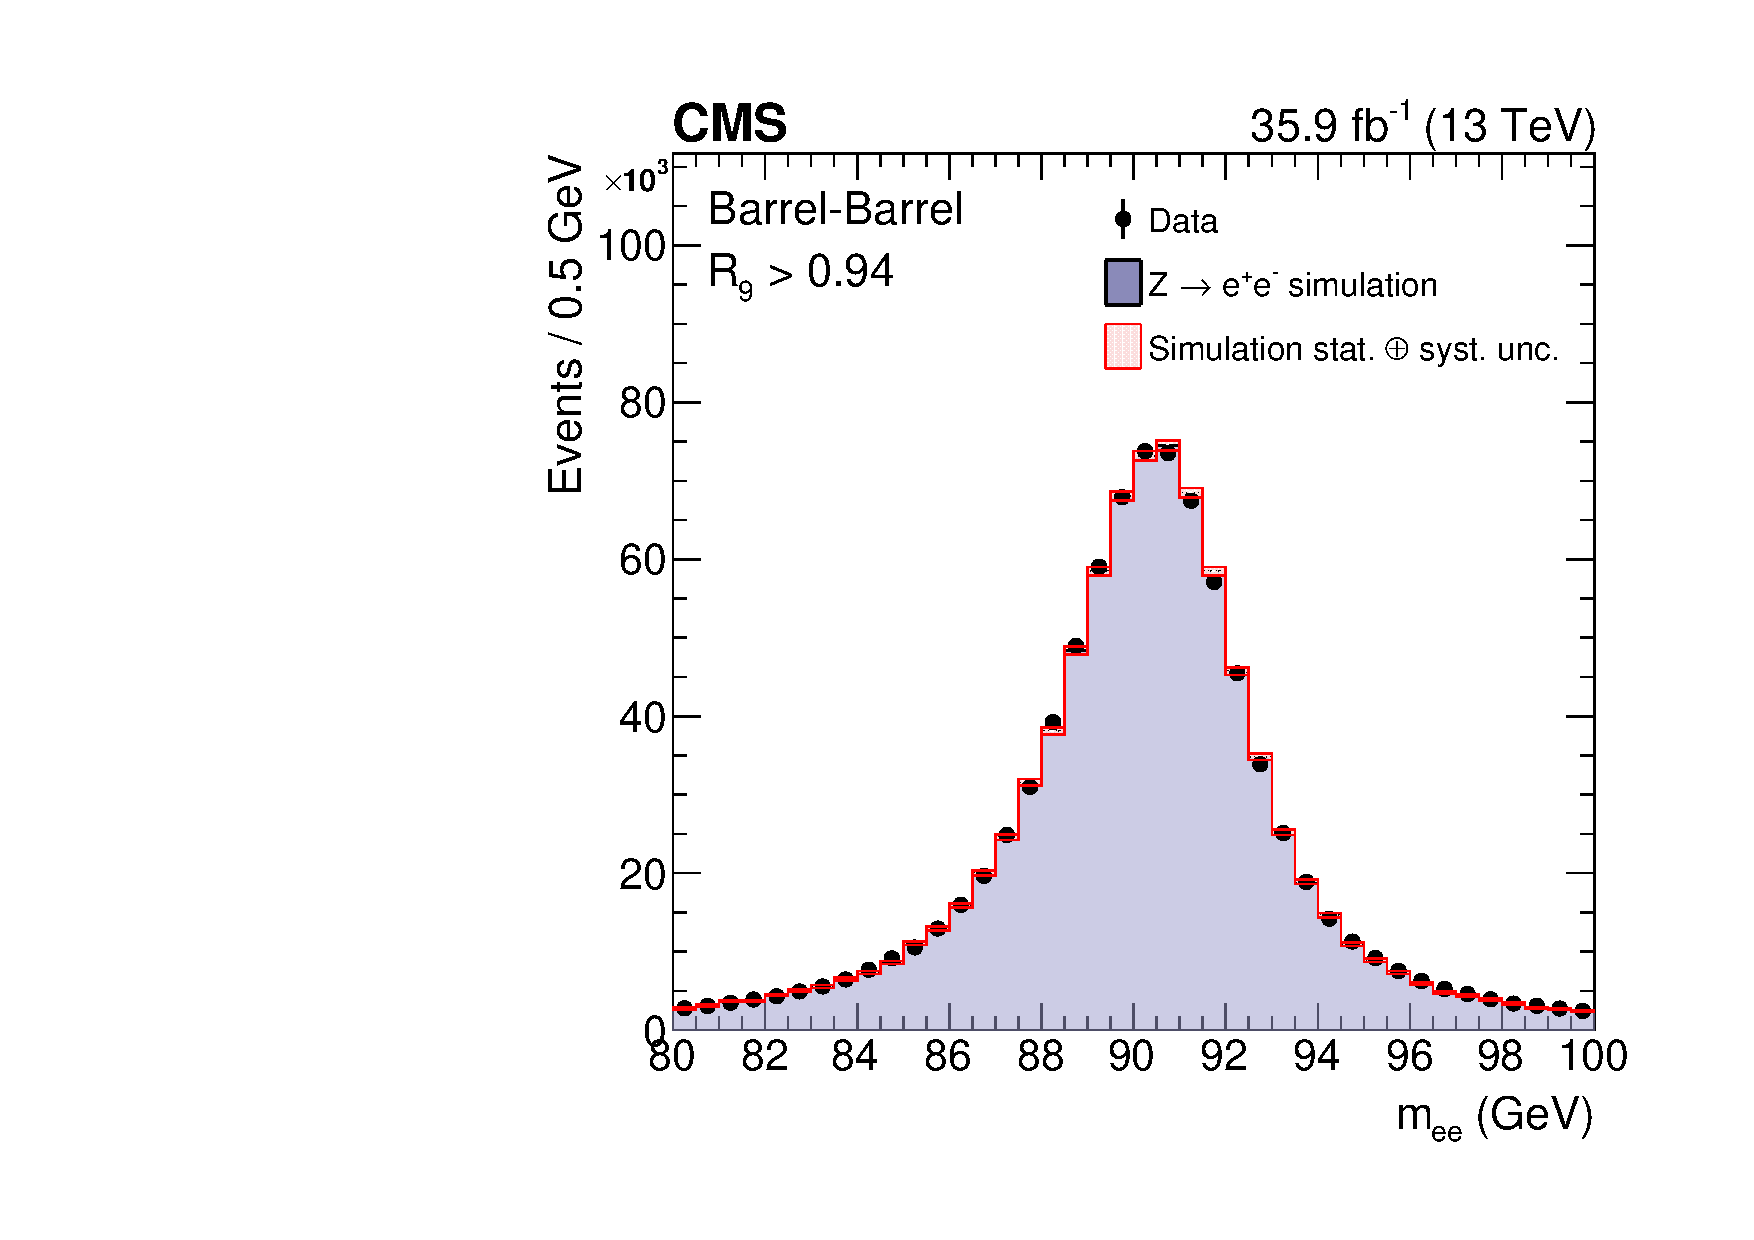
\includegraphics[width=0.5\textwidth]{Fig/ObjReco/Figure_001-a}~
		  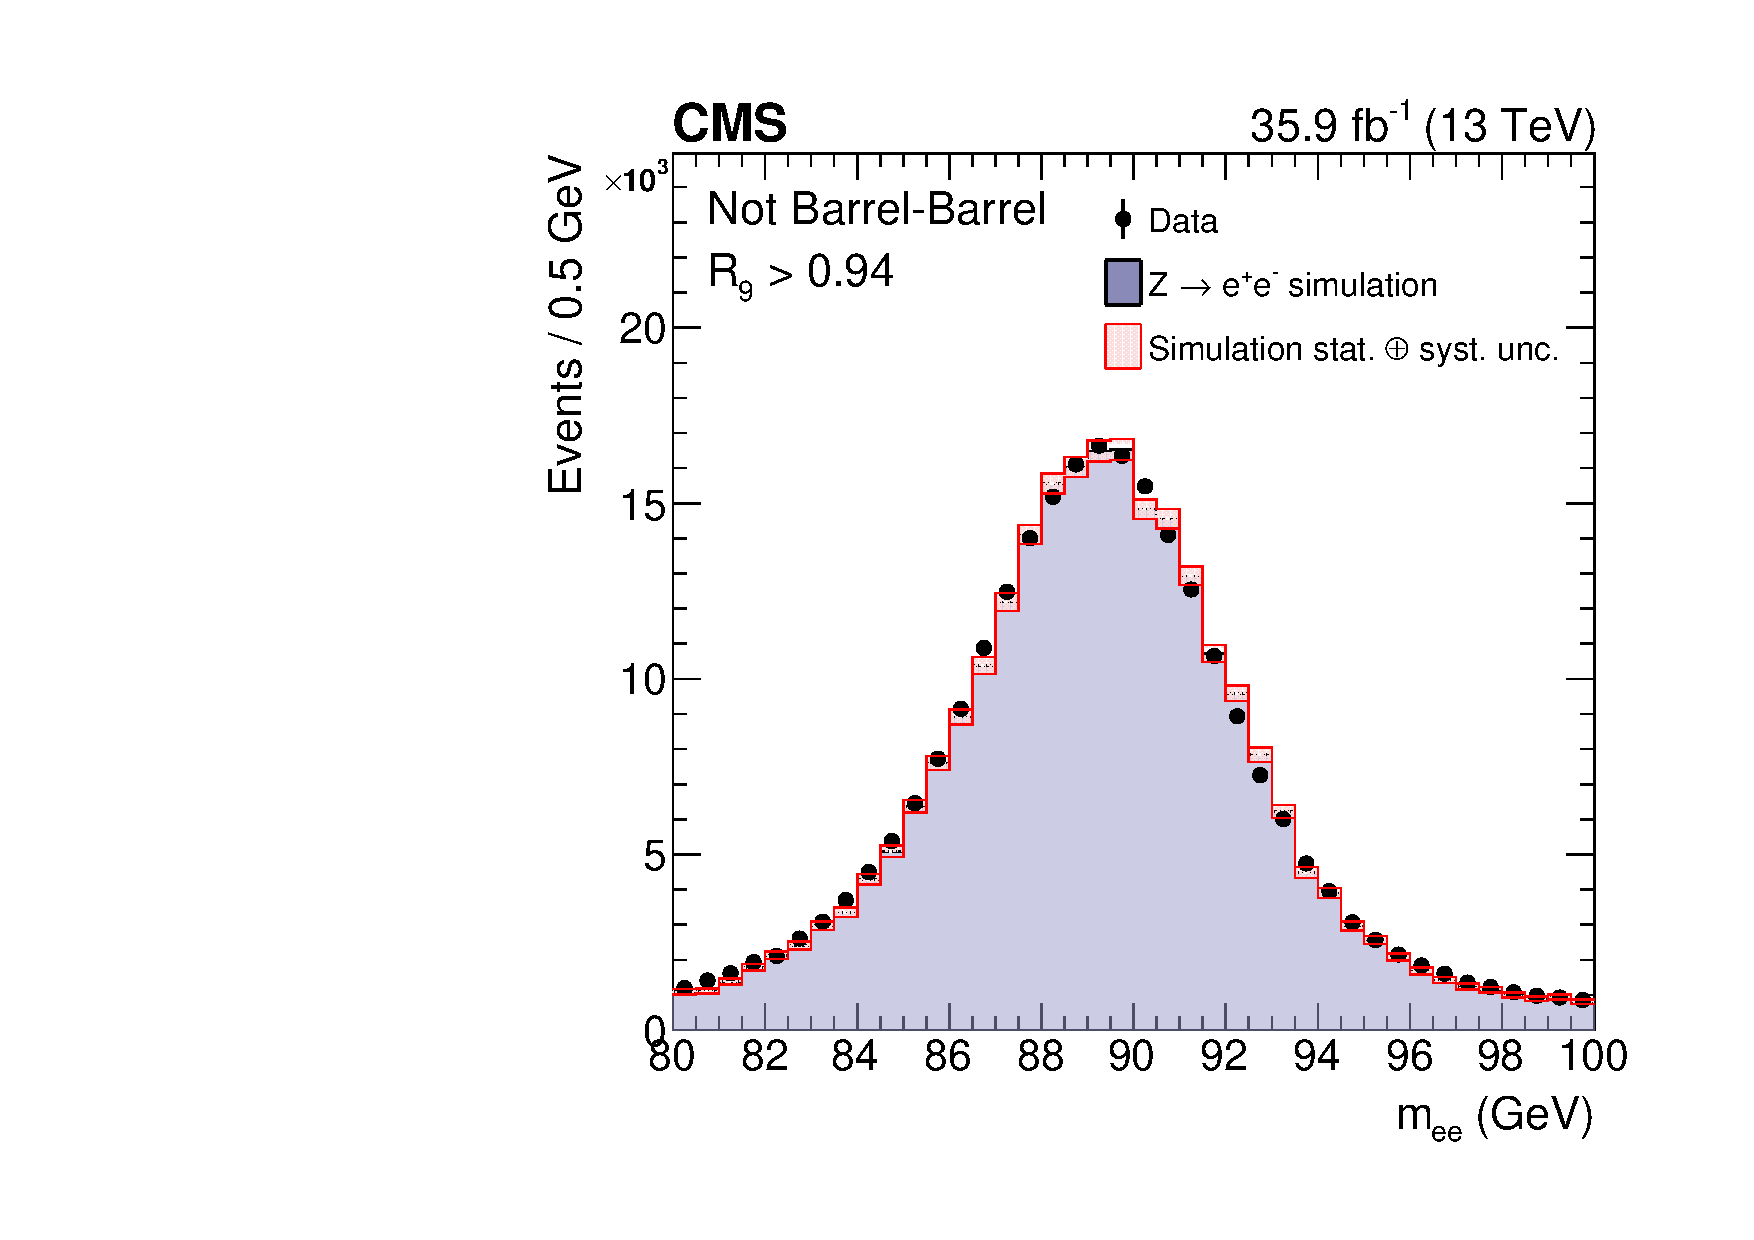
\includegraphics[width=0.5\textwidth]{Fig/ObjReco/Figure_001-b}\\
		  \caption{The comparison of the dielectron invariant mass distributions in data and simulation after energy smearing~\cite{Sirunyan:2018ouh}.}
		  \label{fig:ZeeComp}
		\end{figure}
		
		In the barrel section of the ECAL, an energy resolution of about 1\% is achieved for unconverted or late-converting photons in the tens of \GeV energy range. The remaining barrel photons have a resolution of about 1.3\% up to a pseudorapidity of $\abs{\eta} = 1$, rising to about 2.5\% at $\abs{\eta} = 1.4$. In the endcaps, the resolution of unconverted or late-converting photons is about 2.5\%, while the remaining endcap photons have a resolution between 3 and 4\%~\cite{CMS:EGM-14-001}.		

		\subsection*{Muon reconstruction}
		The muon reconstruction starts with hits in DTs, CSCs and RPCs. Those hits are combined to form segments. This step is called local reconstruction. Three collections of muons reconstructed by different methods are described as follows:
		%The tracks of muons are first reconstructed in the central tracker (referred to as tracker track) and in the muon system (referred to as standalone-muon track) independently, then two methods are used:
		\begin{itemize}
		\item \textbf{Standalone Muon reconstruction}. The segments are used to generate the seeds including the information of positions, directions, and estimated muon $\pt$. The segments and hits from DTs, CSCs and RPCs with the seeds are then fitter by the Kalman-filter technique~\cite{Fruhwirth:1987fm}. The resulting objects are referred to as standalone muon. 
		\item  \textbf{Global Muon reconstruction}.  Each standalone muon track is matched 'outside-in' to a tracker track (also referred to as inner track or silicon track). This global muon track is then fitted by combining the hits from both tracker and standalone tracks using Kalman-filter technique. 
		\item  \textbf{Tracker Muon reconstruction}. Tracker tracks with $\pt>0.5\GeV$ and total momentum $p>2\GeV$ are matched 'inside-out' to the muon system, with bending effect from magnetic field, multiple scattering and expected energy losses while traveling through the detector materials taking into account. The extrapolated track will be considered as tracker muon if it matches to at least one muon segment, formed by hits within each DT and CSC.
		\end{itemize}
%		\begin{figure}[!ht]
%		        \centering
%		    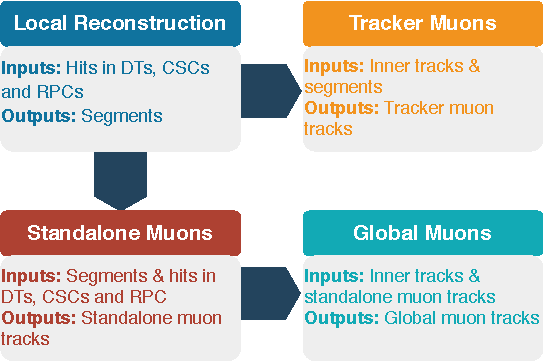
\includegraphics[width=0.7\textwidth]{Fig/MuonRecoDiagram_v1}
%		    \caption{\label{fig:MuonRecoScheme} A schematic diagram to summarize the muon reconstruction.}
%		\end{figure}
		In general, tracker muon reconstruction is more efficient than the global muon reconstruction at low momenta $p\leq 5\GeV$, as it merely requires a single muon segment in the muon system. The downside is that the hadron shower with high energy may ``punch through`` the calorimeter and reach the innermost muon station, which is then misidentified as a tracker muon.  As for the global muon reconstruction, high efficiency is maintained for muons with higher $\pt$, which can traverse through more than one muon station. As a result, around 99\% of muons within the acceptance of the muon system can be well reconstructed either as global muon or tracker muon, and usually as both. For those only reconstructed as standalone muon, they are usually not used in physics analyses as they have worse momentum resolution and are more probable from cosmic-ray. 
		
		The ensemble of reconstructed muons (abbreviated as reco muon) is used as ingredient by the PF event reconstruction. In the PF algorithm, some of identification requirements together with the measurement of energy in the calorimeter are optimized to identify muons with high efficiency and low fake rate, especially those in jets as fake or missed reconstructed (identified) muons can bias measurements of jets and missing transverse energy $\MET$. 
		Consequently, this selection is able to retain not only isolated muons but also non-isolated muons, and those from decay products of hadron that typically treated as background.
		
		Three sets of requirements are imposed to label reco muons as ``isolated``, ``pf-tight``, and ``pf-loose``, and are grouped as particle-flow muons. Reco muons are considered to be isolated if the sum of the $\pt$ of the tracks and of the transverse energy of the calorimeter hits calculated in a cone of size $\Delta R=0.3$ centered on the muon is less than 10\% of the muon $\pt$. The pf-tight and pf-loose selections, tuned to identify muons in jets, are applied to the remaining reco muons. The pf-tight criteria requires the muon track to have a certain number of hits with compatibility with the muon segment and the energy deposited in calorimeter, defined by a template-based simulation. In the pf-loose selection the required number of hits are relaxed and the compatibility requirements are simply replaced to a matching of the track to hits in the muon stations. 
		
		Matching muons to tracks measured in the silicon tracker results in a relative transverse momentum resolution, for muons with \pt up to 100\GeV, of 1\% in the barrel ($\lvert\eta\rvert < 0.9$) and 3\% in the endcaps ($\lvert\eta\rvert > 0.9$). The \pt resolution in the barrel is better than 7\% for muons with \pt up to 1\TeV~\cite{Sirunyan:2018fpa}. The improvement compared to the 2010 results~\cite{Chatrchyan:2012xi} is primarily due to the improvement to the tracker alignment~\cite{Chatrchyan:2014wfa}. 
		
		\subsection{Pile-up \& Primary vertex}
		The high instantaneous luminosity of the LHC results in multiple proton-proton interactions per bunch crossing, which is often referred to as event pile-up. In 13\TeV collisions in 2016 data-taking period, there was on average 27 interactions per bunch crossing, as shown in Fig.~\ref{fig:MeanPU}~\cite{CMSLUMI}.
		
		\begin{figure}[!ht]
		        \centering
		    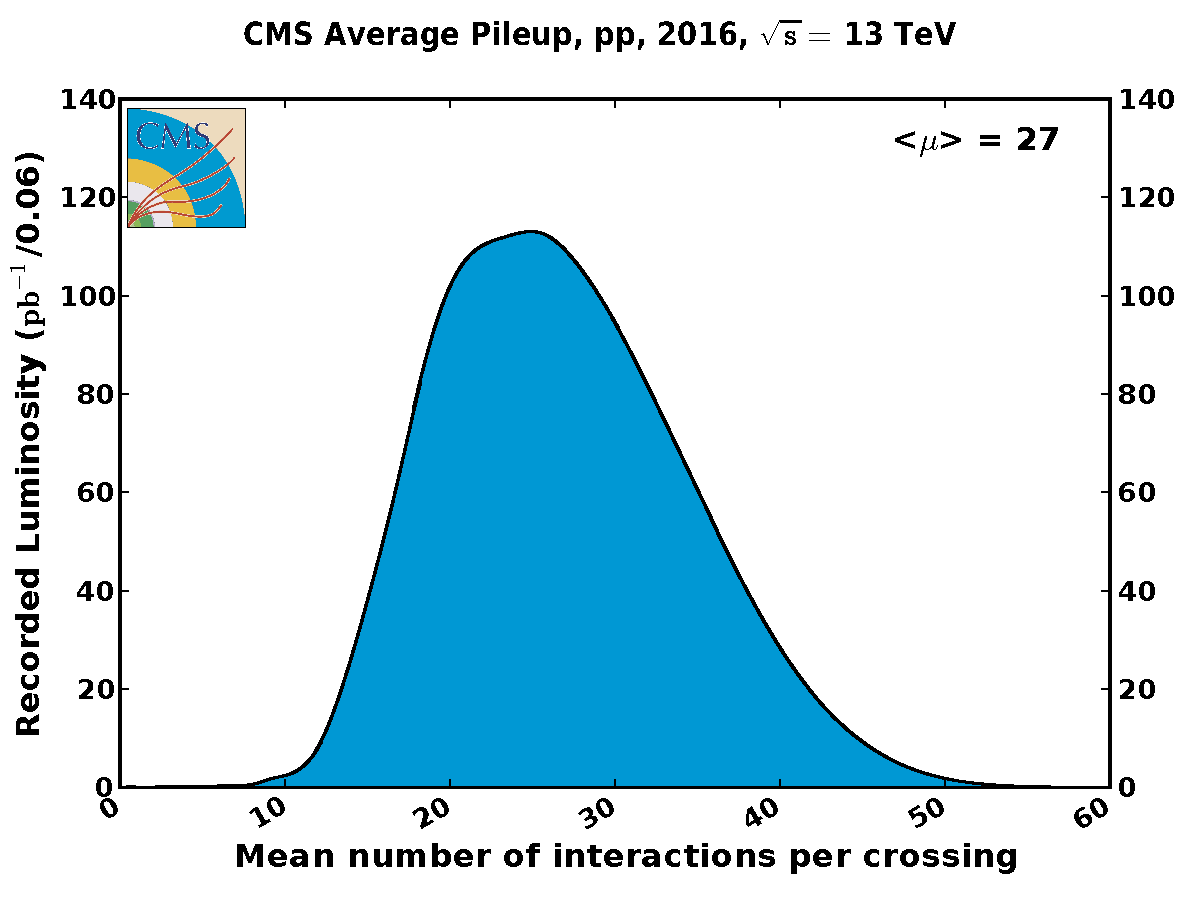
\includegraphics[width=0.6\textwidth]{Fig/pileup_pp_2016}
		    \caption{\label{fig:MeanPU} Mean number of interactions per bunch crossing for the 2016 pp run at 13 \TeV~\cite{CMSLUMI}.}
		\end{figure}
		
	The reconstructed vertex with the largest value of summed physics-object $\pt^2$ is taken to be the primary $\Pp\Pp$ interaction vertex. The physics objects are the jets, clustered using the jet finding algorithm~\cite{Cacciari:2008gp,Cacciari:2011ma} with the tracks assigned to the vertex as inputs, and the associated missing transverse momentum, taken as the negative vector sum of the $\pt$ of those jets.
		The simulated $t\bar{t}$ events (inclusive decays) are used to validate the performance of the vertexing algorithm. Consequently, a resolution, defined as the difference between the position of the reconstructed vertex and the true vertex along the z direction, better than 1\unit{mm} can be achieved, and a harder $\pt$ threshold ($\pt\ _{,min}$) for a track to be taken into account does not result in a significantly degradation of the resolution.
		The efficiency of reconstructing the primary vertex within 5 mm of the true vertex is $\sim 97\%$. Restricting it to be within 1 mm of the generated vertex, the efficiency is about 90\% for $\pt\ _{,min} = 2\GeV$, and remains at $\sim 86\%$ with $\pt\ _{,min} = 5\GeV$~\cite{Contardo:2020886}.